% Options here are passed to the article class.
% Most common options: 10pt, 11pt, 12pt
\documentclass[10pt]{datasheet}

% Input encoding and typographical rules for English language
\usepackage[utf8]{inputenc}
\usepackage[english]{babel}
\usepackage[english]{isodate}

% tikz is used to draw images in this example, but you can
% also use \includegraphics{}.
\usepackage{graphicx}

% These define global texts that are used in headers and titles.
\title{ES01: Palla Encoded V3.100}
\author{PallaPalla}
\tags{encoded-systems, palla}
\date{December 2022}
\revision{Revision 1}

\begin{document}
\maketitle

\section{Features}

\begin{itemize}
\item{Incomplete.}
\end{itemize}

\section{Applications}

\begin{itemize}
\item{Learning about encoded systems}
\end{itemize}

\section{General Description}

TODO
% Switch to next column
\vfill\break

\begin{figure}[h]
    \centering
    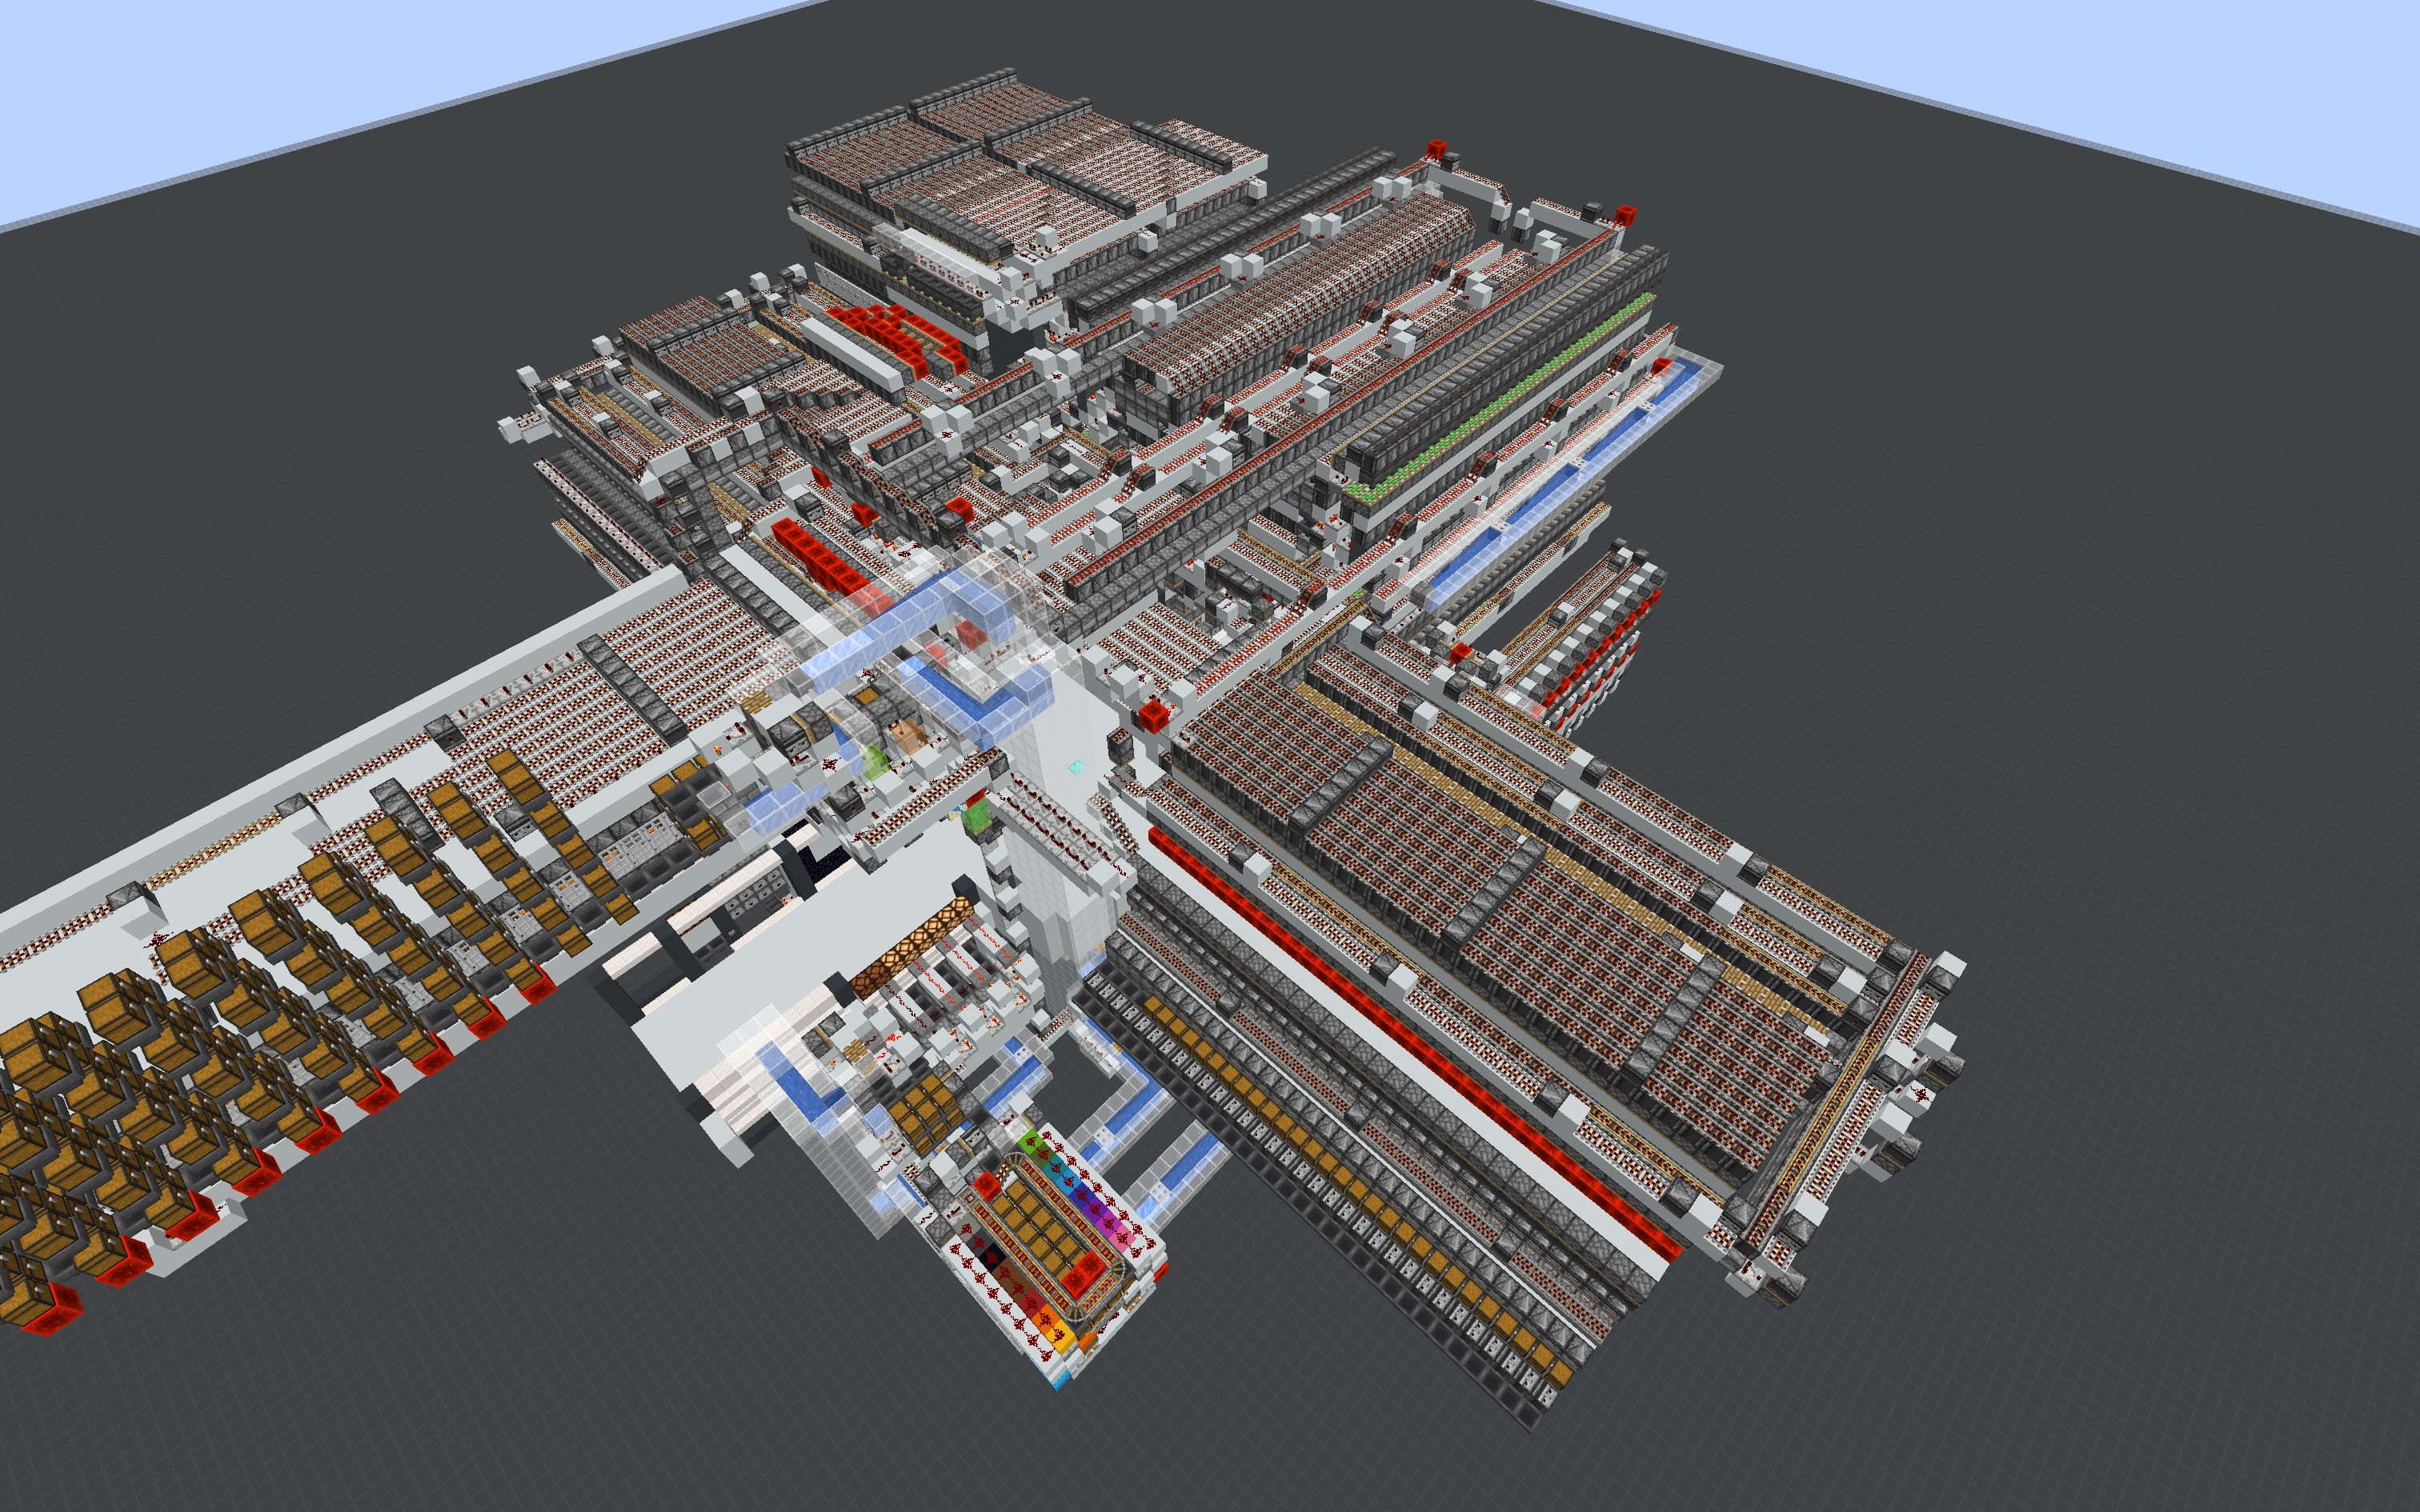
\includegraphics[width=0.48\textwidth]{palla3.1.png}
    \caption{\centering DHQS03 Quad Display Slice}
\end{figure}

% For wide tables, a single column layout is better. It can be switched
% page-by-page.
\onecolumn

\section{Device Specifications}

\begin{table}[h]
    \caption{Device Specifications}
    \begin{tabularx}{\textwidth}{l | c c c | c | X}
        \thickhline
        \textbf{Parameter} & \textbf{Min.} & \textbf{Typ.} & \textbf{Max.} &
        \textbf{Unit} & \textbf{Conditions} \\
        \hline
        MC Version & 1.12 & 1.12.2 & 1.12.2 & MCV & Latest version at time of writing: 1.19.3\\
        \thickhline
\end{tabularx}
\end{table}
\newpage

\section{Download Information}
\begin{table}[h]
    \caption{Download Information}
    \begin{tabularx}{\textwidth}{l | l | l | X}
        \thickhline
        \textbf{Identifier} & \textbf{MC} & \textbf{File} & \textbf{Description} \\
        \hline
        ES01 & 1.12.2 & \href{https://github.com/Soontech-Annals/Archive/blob/364bde8dbcbc2e5337489ff435bcda9b387017e2/Archive/encoded-systems/ES01\%20Palla\%20Encoded\%20V3.100/ES01\_V3.100.schematic?raw=1}{ES01\_V3.100.schematic} & Schematic of system. \\
        \hline
        \thickhline
    \end{tabularx}
\end{table}

\end{document}

